\section{Was ist ein Bild?}
    \subsection{Definition}
        \begin{minipage}[t]{0.45\linewidth}
            \mtitle{\underline{digitale/diskrete Sicht}}
            \begin{center}
                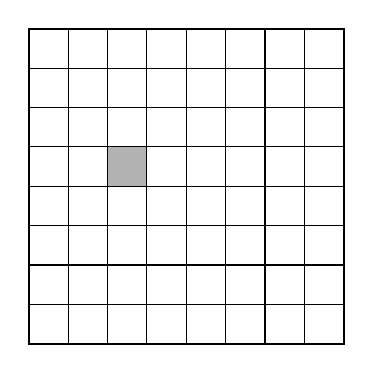
\begin{tikzpicture}
                    \fill[black!30!white] (1,2) rectangle (1.5,2.5);
                    \draw[step=0.5,thin,draw=black] (0,0) grid (4,4);
                    \draw[thick] (0,0) rectangle (4,4);
                \end{tikzpicture}
                \captionof{figure}{Diskretes Bild}
                Darstellung als Matrix.
            \end{center}
        \end{minipage}
        \hfill\vrule\hfill
        \begin{minipage}[t]{0.45\linewidth}
            \mtitle{\underline{kontinuierlich/analoge Sicht}}
            \begin{center}
                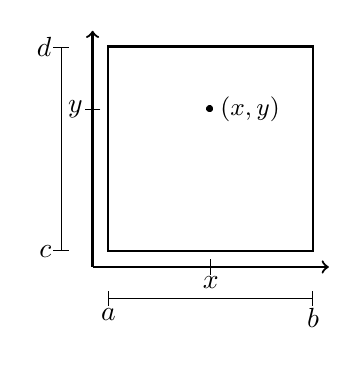
\begin{tikzpicture}
                    \draw[thick,->] (0,0) -- (3,0) ;%node[anchor=west] {X};
                    \draw[thick,->] (0,0) -- (0,3) ;%node[anchor=south] {Y};
                    \draw[thick] (0.2,0.2) rectangle (2.8,2.8);
                    \draw (1.5,2) node[] {\tiny{\textbullet}} node[anchor=west] {\small$(x,y)$};
                    \draw[] (1.5,0.1) -- node[anchor=north] {$x$} (1.5,-0.1);
                    \draw[] (0.1,2) -- node[anchor=east] {$y$} (-0.1,2);
                    \draw[|-|] (0.2,-0.4) node[anchor=north] {$a$} -- (2.8,-0.4) node[anchor=north] {$b$};
                    \draw[|-|] (-0.4,0.2) node[anchor=east] {$c$} -- (-0.4,2.8) node[anchor=east] {$d$};
                \end{tikzpicture}
                \captionof{figure}{Kontinuierliches Bild}
                Darstelllung als Funktion in zwei Veränderlichen
            \end{center}
        \end{minipage}

        \begin{minipage}[t]{0.47\linewidth}
            \pa{Werkzeuge:} Lineare Algebra
            \pa{Vorteile:} Endlicher Speicher
            \pa{Nachteile:} Probleme bei zoomen und drehen
        \end{minipage}
        \hfill\vrule\hfill
        \begin{minipage}[t]{0.47\linewidth}
            \pa{Werkzeuge:} Analysis
            \pa{Vorteile:} Mehr Freiheit (z.b. Kante=Linie entlang einer Unstetigkeit)
            \pa{Nachteile:} Unendlicher Speicher
        \end{minipage}

        \begin{definition*}
            Ein \textbf{Bild}\index{Bild} ist eine Funktion $u: \Omega \to F$, wobei $\Omega \subset \mathbb Z^d$ (im diskreten Fall) oder $\Omega \subset \mathbb R^d$ (im kontinuierlichen Fall).
            \begin{enumerate}
                \item[$d=2$:] Typisches 2D Bild
                \item[$d=3$:] 3D-Bild bzw. "Körper" \ \underline{oder} Video: 2D Ort + Zeit
            \end{enumerate}
            F ist der \textbf{Farbraum}\index{Farbraum}, Beispiele:
            \begin{enumerate}[label=\textbullet]
                \item F$=[0,1]$ oder F=$\{0,1,..., 255\}$, Graustufen
                \item F$=\{0,1\}$ schwarz/weiß
                \item F$=[0,1]^3$ oder F$=\{0,1,...,255\}^3$ Farbbilder
            \end{enumerate}
        \end{definition*}
    \subsection{Umwandlung}

        \pa{kontinuierlich $\to$ diskret:}\\
            \begin{minipage}[t]{0.4\linewidth}
                \
                \begin{center}
                    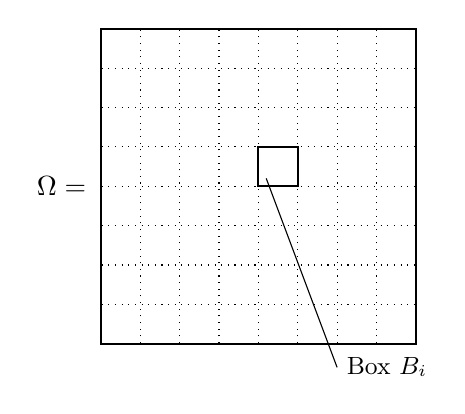
\begin{tikzpicture}
                        \draw (-0.5,2) node {$\Omega=$};
                        \draw[step=0.5,thin,draw=black,dotted] (0.01,0.01) grid (3.99,3.99);
                        \draw[thick] (0,0) rectangle (4,4);
                        \draw[thick] (2,2) rectangle (2.5,2.5);
                        \draw[] (2.1,2.1) -- (3,-0.3) node[anchor = south west, yshift = -7] {\small Box $B_i$};
                    \end{tikzpicture}
                \end{center}
            \end{minipage}
            \hfill\vrule\hfill
            \begin{minipage}[t]{0.59\linewidth}
                \
                \begin{center}
                    \begin{enumerate}[label=\textbullet]
                        \item $\Omega$ in Gitter zerlegen.
                        \item Jede Box durch nur einen Farbwert approximieren.
                        \item Etwa durch den Funktionswert im Mittelpunkt der Box.
                        \item oder durch den Mittelwert in der Box: 
                            \[
                                \displaystyle \frac{1}{\abs{B_i}} \C \int_{B_i}u(x)\d x.
                            \]
                    \end{enumerate}
                \end{center}
            \end{minipage}

                \ \\
            \pa{Diskret $\to$ Kontinuierlich:}\\
                \begin{minipage}[t]{0.4\linewidth}
                    \
                    \begin{center}
                        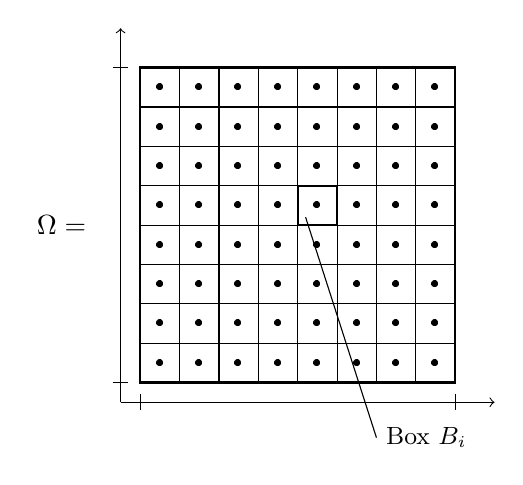
\begin{tikzpicture}
                            \draw (-1,2) node {$\Omega=$};
                            \draw[->] (-0.25,-0.25) -- (-0.25,4.5);
                            \draw[->] (-0.25,-0.25) -- (4.5,-0.25);
                            \draw (-0.35,4) -- (-0.15,4);
                            \draw (-0.35,0) -- (-0.15,0);
                            \draw (0,-0.35) -- (0,-0.15);
                            \draw (4,-0.35) -- (4,-0.15);
                            \draw[step=0.5,thin,draw=black] (0,0) grid (4,4);
                            \foreach \x in {0.25,0.75,..., 3.75}{
                                \foreach \y in {0.25,0.75,..., 3.75}{
                                    \draw (\x,\y) node {\tiny \textbullet};
                            }
                            }
                            \draw[thick] (0,0) rectangle (4,4);
                            \draw[thick] (2,2) rectangle (2.5,2.5);
                            \draw[] (2.1,2.1) -- (3,-0.7) node[anchor = south west, yshift = -7] {\small Box $B_i$};
                        \end{tikzpicture}
                    \end{center}
                \end{minipage}
                \hfill\vrule\hfill
                \begin{minipage}[t]{0.59\linewidth}
                    \
                    \begin{center}
                        \begin{enumerate}
                            \item[1.] Idee: Jeder Punkt der Box $B_i$ erhält den Funktionswert von $B_i$ als Farbwert\\
                                $\Rightarrow$ \textbf{Nearest neighbour Interpolation}\index{Nearest neighbour Interpolation}.
                            \item[2.] Idee: Mittelpunkt von Box $B_i$ erhält den Wert von Pixel $B_i$ sonst wird interpoliert.\\
                            Grauwert $g \coloneqq $ Gewichtetes Mittel aus Grauwerten $a,b,c,d$.\\
                        \end{enumerate}

                            \begin{center}
                                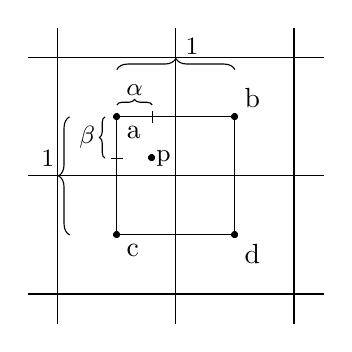
\begin{tikzpicture}[scale=1.5]
                                    \draw[step = 1] (0.75,0.75) grid (3.25,3.25);
                                    \foreach \x in {1.5,2.5}{
                                        \foreach \y in {1.5,2.5}{
                                            \draw (\x,\y) node {\tiny \textbullet};
                                    }
                                    }
                                    \draw (1.5,2.5) node[anchor=north west] {a};
                                    \draw (2.5,2.5) node[anchor=south west] {b};
                                    \draw (1.5,1.5) node[anchor=north west] {c};
                                    \draw (2.5,1.5) node[anchor=north west] {d};

                                    \draw (1.5,1.5) rectangle (2.5,2.5);
                                    \draw (1.45,2.15) -- (1.55,2.15);
                                    \draw (1.8,2.45) -- (1.8,2.55);
                                    \draw[decorate,decoration={brace,amplitude=2pt}] (1.5,2.6) -- node[anchor=south] {\small $\alpha$} (1.8,2.6);
                                    \draw[decorate,decoration={brace,amplitude=2pt}] (1.4,2.15) --node[anchor=east] {\small $\beta$} (1.4,2.5);
                                    \draw (1.8,2.15) node {\tiny \textbullet} node[anchor=west, xshift=-2] {\small p};
                                    \draw[decorate,decoration={brace,amplitude=4pt}] (1.5,2.9) -- node[anchor= south west,yshift = 2] {\small 1} (2.5,2.9);
                                    \draw[decorate,decoration={brace,amplitude=4pt}] (1.1,1.5) -- node[anchor= south east, xshift=-2] {\small 1} (1.1,2.5);
                                \end{tikzpicture}
                            \end{center}

                            \small{$g=(1-\alpha)  (1-\beta)  a + \alpha  (1- \beta)  b + (1-\alpha)  \beta  c + \alpha  \beta  d$}\\
                            Dieses wird \textbf{Bilineare Interpolation}\index{Bilineare Interpolation} genannt.
                    \end{center}
                \end{minipage}

    \subsection{Beispiel Rotation}
        \begin{center}
            \begin{tikzpicture}%TODO redo
                \draw (0,0.1) -- node[anchor=center] {\tiny \textbullet} node[anchor=north] {\tiny $0$} (3,0.1);
                \draw  (4,0.1) node  {$\overset{\text{\footnotesize um $\alpha$ drehen}}{\implies}$};
                \draw (6.5,0.1) -- ++(30:1.5);
                \draw (6.5,0.1) node[anchor=center] {\tiny \textbullet} node[anchor=north] {\tiny $0$} -- ++(210:1.5);
                \draw[dotted] (5,0.1) -- (8,0.1);
                \draw (7,0.1) arc[radius=0.5,start angle=0,end angle=30]  node[anchor = north west] {\tiny $\alpha$};
            \end{tikzpicture}
        \end{center}

        \pa{1. Fall, kontinuierliches Bild}\\
        Sei $u$ das alte Bild und $v$ das neue Bild, dann ist die Drehung gegeben durch eine \textbf{Drehmatrix}\index{Drehmatrix}:

            \[D_\varphi \in \R^{2 \times 2}, D_\varphi=\mat{\cos(\varphi) \ -\sin(\varphi) \\ \sin(\varphi) \ \cos(\varphi)}\]

            Damit folgt, dass $D(u)= D_\varphi \Omega$ und $v(x)=u(\underbrace{D_\varphi^{-1}x}_{\in \Omega}) = u(D_{-\varphi}x)$. ($D(u)$ ist die \textbf{Domain}\index{Domain} von $u$)

        \pa{2. Fall, diskretes Bild}\\
        Dieses ist problematisch, denn i.A.\@ $D_{-\varphi} x \not \in \Z^2$ für $x \in \Z^2$.

            \begin{center}
                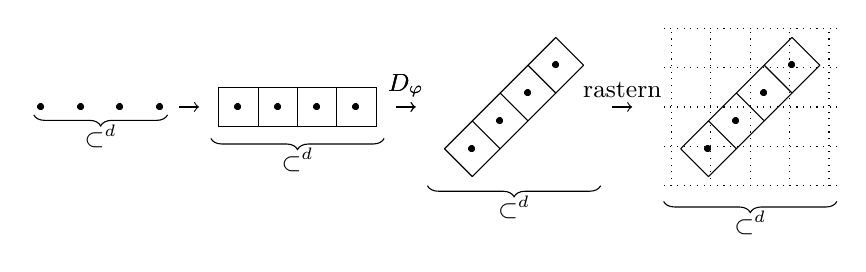
\begin{tikzpicture}
                    \foreach \x in {0,1,2,3}{
                            \draw (0.5*\x,0) node {\tiny \textbullet};
                    }
                    \draw[decorate,decoration={brace,amplitude=4pt,mirror}] (-0.1,-0.1) -- node[anchor= north] {\small $\subset \Z^d$} (1.6,-0.1);
                    \draw[->] (1.75,0) -- (2,0);
                    \draw[step=0.5, shift={(2.25,0.25)}] (0,0) grid (2,-0.5);
                    \foreach \x in {0,1,2,3}{
                        \draw[shift={(2.5,0)}] (0.5*\x,0) node {\tiny \textbullet};
                    }
                    \draw[decorate,decoration={brace,amplitude=4pt,mirror}] (2.15,-0.4) -- node[anchor= north] {\small $\subset \R^d$} (4.35,-0.4);
                    \draw[->] (4.5,0) -- node[above] {\small $D_\varphi$} (4.75,0);
                    \draw[step=0.5, shift={(5,0.25)},rotate around = {45:(1,-0.25)}] (0,0) grid (2,-0.5);
                    \foreach \x in {0,1,2,3}{
                        \draw[shift={(5.25,0)},rotate around = {45:(0.75,0)}] (0.5*\x,0) node {\tiny \textbullet};
                    }
                    \draw[decorate,decoration={brace,amplitude=4pt,mirror}] (4.9,-1) -- node[anchor= north] {\small $\subset \R^d$} (7.1,-1);
                    \draw[->] (7.25,0) -- node[above] {\small rastern} (7.5,0);
                    \draw[->] (4.5,0) -- node[above] {\small $D_\varphi$} (4.75,0);
                    \draw[step=0.5, shift={(8,0.25)},rotate around = {45:(1,-0.25)}] (0,0) grid (2,-0.5);
                    \foreach \x in {0,1,2,3}{
                        \draw[shift={(8.25,0)},rotate around = {45:(0.75,0)}] (0.5*\x,0) node {\tiny \textbullet};
                    }
                    \draw[dotted,step=0.5] (7.9,1) grid (10.1,-1);
                    \draw[decorate,decoration={brace,amplitude=4pt,mirror}] (7.9,-1.2) -- node[anchor= north] {\small $\subset \Z^d$} (10.1,-1.2);
                \end{tikzpicture}
            \end{center}

            In beiden Fällen: Lasse $x$ durch die Domain von $v$ laufen und setze $v(x) \coloneqq u(D_\varphi^{-1} x)$, wobei der konkrete Wert durch Interpolation bestimmt wird.

            \begin{center}
                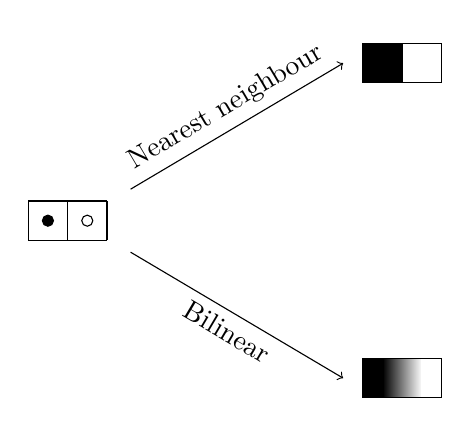
\begin{tikzpicture}
                    \draw[step=0.5, shift={(3,0.25)}] (0,0) grid (1,-0.5);
                    \draw[fill] (3.25,0) circle[radius=2pt];
                    \draw[] (3.75,0) circle[radius=2pt];
                    \draw[->] (4.3,-0.4) -- node[sloped,below] {Bilinear} (7,-2);
                    \draw[->] (4.3,0.4) -- node[sloped,above] {Nearest neighbour} (7,2);
                    \draw[step=0.5, shift={(7.25,2.25)}] (0,0) grid (1,-0.5);
                    \draw[fill] (7.25,2.25) rectangle (7.75,1.75);
                    \fill[draw = white,left color = black, right color = white!100] (7.5,-2.25) rectangle (8,-1.75);
                    \draw[fill,black] (7.25,-2.25) rectangle (7.51,-1.75);
                    \draw[shift={(7.25,-1.75)}] (0,0) rectangle(1,-0.5);
                \end{tikzpicture}
            \end{center}            

